% !TEX root = document.tex

\chapter{\label{chap:statix-compiler}The Statix Compiler}

\section{Compilation pipeline}
In this section we will describe the steps which currently transform the a textual Statix file to a spec file which is compatible with the Statix solver. The pipeline can be seen in Figure \ref{fig:pipeline}.

\begin{figure}[h]
  \centering
  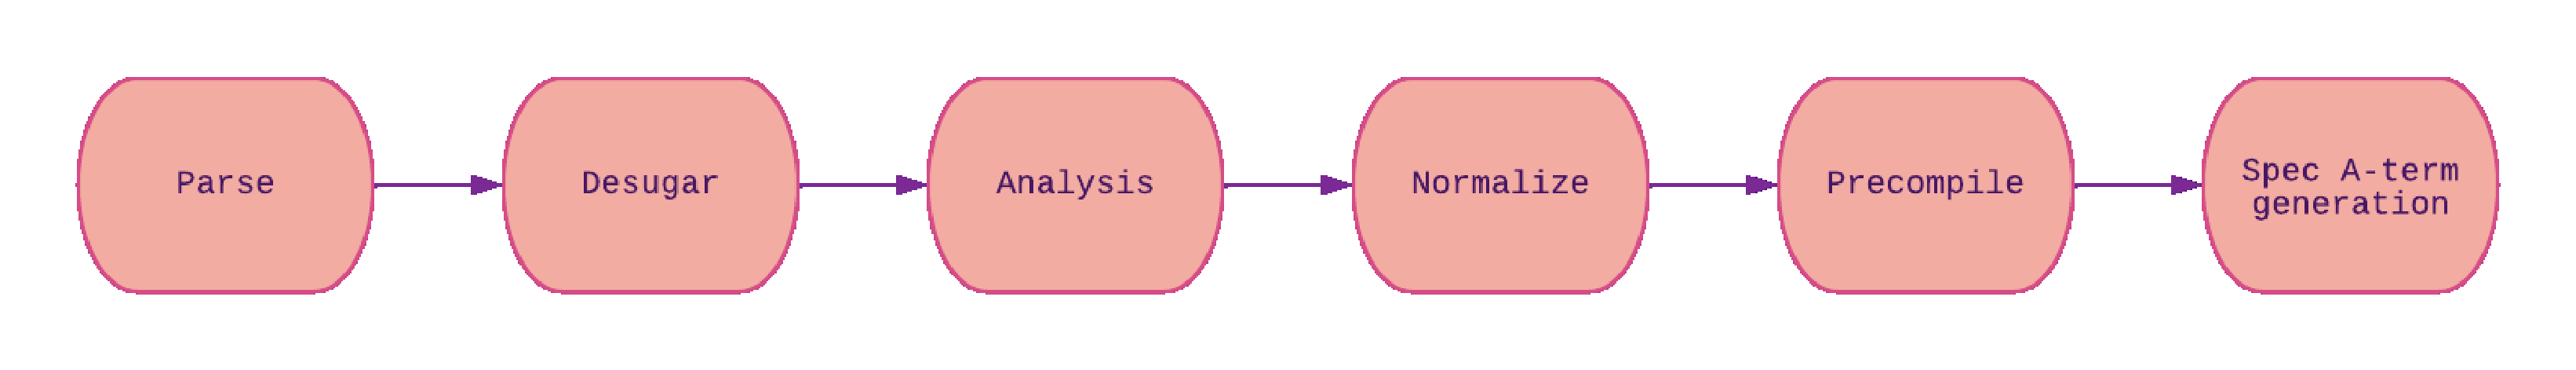
\includegraphics[height=2.3cm]{img/Statix-compiler-pipeline.eps}
  \caption{The Statix compiler pipeline}
   \label{fig:pipeline}
\end{figure}

\begin{itemize}
\item The first step is parsing the text file to an abstract syntax tree (AST) according to its grammar specification in SDF3 ($\mathtt{textfile \to parsed \; AST}$).
\item The next step is the desugaring step in which a subset of the constructs of syntactic sugar get transformed to the core constructs that are supported by the Statix solver ($\mathtt{parsed \; AST \to desugared \; AST}$).
\item After this step static analysis is performed on the AST by combining it with the static semantics specification and solving the constraints. The results of the solver are stored in an analysis object ($\mathtt{desugared \; AST \to analyzed \; AST, \; analysis \; object}$).
\item The type information stored in the analysis object can then be used to transform the remaining sugared constructs to core constructs in the normalization step ($\mathtt{analyzed \; AST,}$ $\mathtt{analysis \; object \to normalized \; AST}$).
\item In addition the analysis object is used to precompile the scope graph queries such as is explained in \textit{reference precompilation paper} ($\mathtt{normalized \; AST, \; analysis \; object \to precompiled \; AST}$).
\item Finally the AST is transformed into the spec A-Term format that is supported by the Statix solver ($\mathtt{precompiled \; AST, \; analysis \; object \to spec \; ATerm \; file}$).
\end{itemize}


\section{Static Analysis}
The static analysis mostly gets done by solving the constraints defined in the specification file. In the current compiler this file is written in the deprecated NaBL2 meta-language, while in the bootstrapped version of the compiler the constraints will be specified in Statix itself.

A large part of the constraint specification concerns the typing of Statix. For example, an arithmetic constraint only allows terms that have the integer type. Another part of the specification is defining how names in Statix are resolved.

\subsection{Custom Analysis}
The majority of the static semantics of Statix can be expressed using the aforementioned meta-languages, but there are some constraints that the meta-languages can't support. An example is checking whether the name of a Statix module corresponds to its file-path, since both NaBL2 and Statix don't have access to this information. To make sure that these kind of static semantics can also be checked, the runtime of the meta-languages allows the designers to write a custom analysis section in the Stratego meta-language, which is a less restricted language used for the manipulation of ASTs.
Checking for overlapping rule patterns and correct scope graph extension behavior are two more complex examples of this custom analysis that we will explain in the following subsections.

\subsection{Overlapping rule patterns}

\subsection{Scope graph extensions}


\section{Normalization}

\section{A-Term generation}